\chapter{Architecture}

\textcolor{blue}{(5-8 pages) Here you will present the architecture or model that you have chosen and that
is (or will be) implemented in your work. Note that putting algorithms in your
report is not desirable but in certain cases these might be placed in the appendix.
Code further be avoided in the report itself but may be delivered in the fashion
requested by the supervisor or, in the case of masters delivery, submitted as
additional documents.}

This section describes the overall architecture and how the system works. First the general system will be described, and then the API Layer and classification server in turn.  

To make the system as modularized and responsive as possible, the API layer was written in Node.js and the sentiment classifier in the Python programming language. Both systems are continuously running servers. This allows multiple services to run simultaneously, both for the API layer and the classifier. The idea is to make the system horizontally scalable.

\begin{figure}[ht]
 \begin{center}
     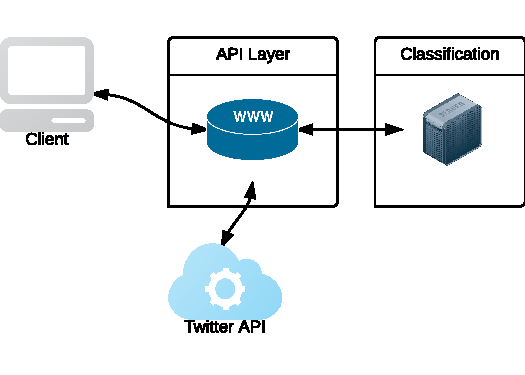
\includegraphics[width=0.8\textwidth]{../img/NetworkDiagram.pdf}
 \end{center}
 \caption[Architectural overview of the system.]{Architectural overview of the system. The client retrieves data from the Twitter API and uses the classification server for sentiment classification.}
 \label{fig:NetworkDiagram.pdf}
\end{figure}

A client makes a request to the API Layer, with the same interface as the Twitter API service. From there the API Layer will retrieve information from the Twitter API with HTTP requests, iterate over all tweets received, and send them in parallel to the classification server. When the classification server is done processing and classifying the tweet, it is sent back to the API Layer. When the API layer has received all the tweets, it responds to the client with the same JSON structure as the Twitter API sends out, only with an additional attribute noting the tweet's sentiment. This architecture and application flow can be seen in~\autoref{fig:NetworkDiagram.pdf}. 

\section{API Layer Extension}

To be able to have a scalable and responsive solution, the API Layer was written using the Node.js platform. Since Node.js uses JavaScript as programming language, the JSON data retrieved from the Twitter REST and Streaming API are easily manipulated and passed around. 

The API Layer works as a thin layer extending the Twitter API. This means that the interface used by Twitter, with all defined options and appropriate methods, is reflected through the API Layer. The main benefit is that all documentation for the Twitter API also documents most of this extended API Layer.

For authentication, an application is registered with a developer account at the Twitter Developer site. This creates OAuth credentials, which is used to identify the application, and to gain access to the Twitter data. For this implementation, the data is retrieved using the OAuth access for the application, not at user level. 

\subsection{Architectural Flow}


\begin{figure}[htb]
 \begin{center}
     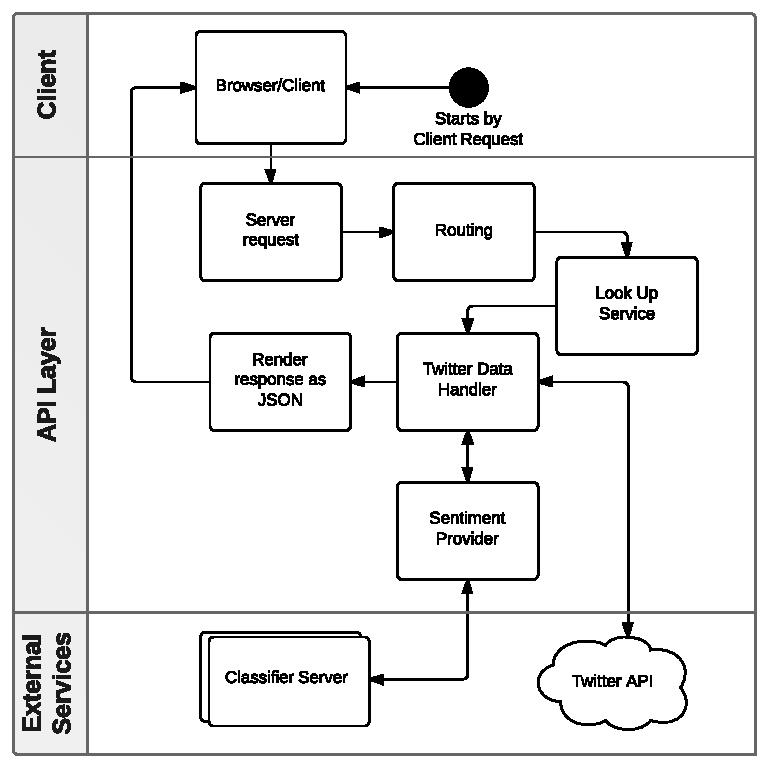
\includegraphics[width=0.8\textwidth]{../img/APILayerArcitechture.pdf}
 \end{center}
 \caption[Architectural overview of the API Layer.]{Architectural overview of the API Layer. A request is handled by the server, sending it to routing where it is processed and sent to service look-up. If a service is found, a request is sent to the Twitter API and the received data is extended by the Twitter Data Handler module to contain a sentiment. When all of the Twitter data are extended, the data is given as a response to the requesting client.}
 \label{fig:APILayerArcitechture.pdf}
\end{figure}

When a request from a client is made, the request gets processed by the server and the routing module determines what the client is looking for. When the proper service is found, the client-specified parameters are sent directly to the Twitter API, using the Twitter Data Handler module (TDH). The TDH module then iterates over all found tweets, and sends them in parallel to the classification server. When a tweet has been processed by the classification server the classified sentiment is sent back to the TBH module and the original tweet object is extended to contain a property with the sentiment. When all tweets are classified, the TBH module passes the extended twitter data to the render module. The render module renders the JSON data and sends it to the client with appropriate HTTP headers set. This application flow can be seen in~\autoref{fig:APILayerArcitechture.pdf}.

If there is an error during any part of the process, the error is caught by the routing module, and the error is rendered as a JSON object, in the same manner as it would be by the Twitter API. 

When using both the Twitter REST API and Streaming API, there is a high level of asynchronism. Especially when streaming, it is impossible to predict when the next tweet is received. Due to this the system designed needs to be able to handle this dynamic data flow. Node.js is an event-driven platform and has a natural support for asynchronous data. 

All internal and external message passing in the API Layer is asynchronous. When requesting Twitter for data, an event is triggered when that data is ready and all tweets are separately sent to the classifier. By sending all tweets separately in parallel, classification of the entire set of tweets does not take much longer than classifying only one tweet. 

When streaming, the TBH module opens a connection to the Twitter API, but never closes it. There is a continuously open connection to the Twitter server, which is feeding the TBH module with single tweets as they get stored in the Twitter system. From the first received tweet, a connection to the requesting client is opened by the render response module. This connection will also remain open. In this way there is an open connection between the client and the API Layer as well as between the API Layer and the Twitter API. The API Layer works as a middleman, taking in tweets, classifying them, and streaming them to the client. By running this entire process asynchronously, the system can process data independently of when it is published.


\section{Sentiment Analysis Classifier}

Python is computationally stronger than Node.js in many ways. Additionally, it is much more mature. There are a lot of stable, well documented, packages for handling various tasks. Natural Language Toolkit (NLTK) is one of these packages. NLTK is a widely used package for natural language processing and has integrated modules to handle well-known techniques such as lexica and n-gram feature selection. Thus it is a good choice for the process of sentiment analysis. As a dynamic typed language, Python also allows for rapid development and prototyping. These attributes are some of the reasons Python is a good fit for the present system. 

The Sentiment Analysis Classifier system runs as a server waiting for requests. The HTTP method POST is used for a client to send a \textit{stringified} tweet object to the server. Stringify is a JSON method for returning a serialized object represented by a string. The classification server converts this string to a Python dictionary. The response will be a string with the sentiment classification, that is, either \textit{positive}, \textit{neutral} or \textit{negative}. The classification scheme can be extended if necessary. 

The classifier server can be initialized with different settings for classification strategy, what port to run at, what training data to use, and whether or not to show debug data. This allows for multiple servers running at the same time, with different settings. Running multiple server instances makes it easier to compare different classification strategies. Two servers could run side by side, and a test framework could use the two servers to classify the same tweets for a comparison.

The classification server uses a pool of child processes. For each receiving tweet, it spawns a new child from this pool and in this process the tweet is classified. This way the classification server can process several tweets in parallel, which helps the one-to-one relationship between a tweet on the classification server and the same tweet on the API Layer.

\subsection{Architectural Flow}

\begin{figure}[htb]
 \begin{center}
     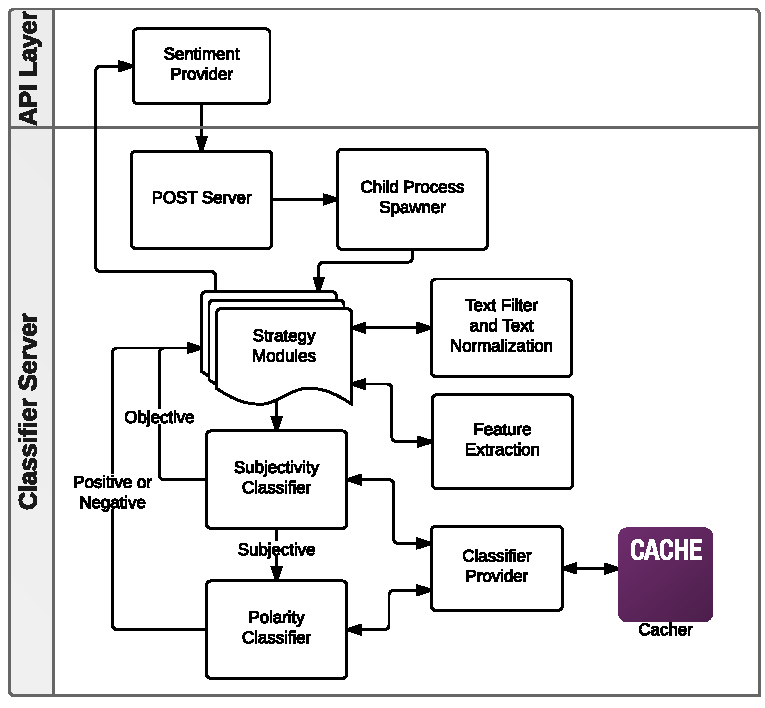
\includegraphics[width=0.8\textwidth]{../img/ClassifierArcitechture.pdf}
 \end{center}
 \caption[Architectural overview of the classification server.]{Architectural overview of the classification server. The API Layer makes a request to the POST Server. Child processes are spawned per received tweet. Different Strategy Modules can be implemented and used. The strategies can use several text filters, normalization and feature extractions. The strategies use both the subjectivity and polarity module to classify the tweet. If the tweet is classified as subjective, the classification is handed to the strategy module, if not, the tweet is sent to the polarity classifier. After classifying the tweet, the polarity classifier returns the classification to the strategy module.}
 \label{fig:ClassifierArcitechture}
\end{figure}

The Sentiment Provider module from the API Layer makes a request to the classifier's POST Server. The POST server translates the string to a Python dictionary and passes the information down to the Child Process Spawner. A new process is spawned using the strategy specified when initiating the server. 

The strategy modules use various text filters, normalizations and feature extraction methods, depending on the selected strategy. The strategy modules can choose to have different filters and features for both the subjectivity classifier and the polarity classifier. 

The strategy modules send the features to the subjectivity classifier. This module classifies the tweet according to whether it is subjective or objective. Both classification types use the classifier provider to retrieve a possible trained classifier. If no cached trained classifier exists, the classifier provider trains a classifier and caches the result for easier access at the next execution. 

The subjectivity classifier will return a response to the strategy module, which in turn will return data to the API Layer, if the tweet gets interpreted as objective. This stops the classification cycle. However, if the tweet is classified as subjective, it is passed on to the polarity classifier module. 

The polarity classifier works in a similar manner as with the subjectivity classifier. It uses the classifier provider to retrieve a classifier with the selected parameters. The polarity classifier provides the strategy module with the finished classification string.


\subsection{Current Implementation}

The current implementation uses a simpler form than the architecture described above. The classification is a simple, basic, approach. It does not use any machine learning. It uses the AFINN lexicon by~\cite{article:afinn} to calculate sentiment strength. The sentiment is then returned directly to the API Layer's Sentiment Provider, without using the subjectivity or polarity classifiers.

The strategy modules have most of the responsibilities of the system. To explore different techniques for doing sentiment analysis, a new strategy module can be developed using existing code for filtering and feature extraction. 
